\documentclass[12pt]{article}
%--------------------   start of the 'preamble'
%
\usepackage{graphicx,amssymb,amstext,amsmath,color}
\usepackage[margin=2cm]{geometry}
\usepackage{abstract}
\usepackage{setspace}
\usepackage[footnotesize,bf]{caption}

% TABLE
\usepackage{multicol,hhline,colortbl,multirow}
\usepackage{braket}
\usepackage{siunitx}
\usepackage{hyperref}
\usepackage{authblk}
\usepackage{siunitx}
\usepackage{mathrsfs}
%%\usepackage[sort&compress]{natbib}
%%\bibpunct{(}{)}{,}{a}{, }{;}
%
\usepackage[sort&compress]{natbib}
\bibpunct{[}{]}{,}{s}{}{;}


\definecolor{gray}{gray}{0.8}
\def\mobunits{\square\centi\meter\per\volt\per\second}
\def\gcm{\gram\per\cubic\centi\meter}
\def\ccg{\cellcolor{gray}}

\renewcommand{\labelitemii}{$\circ$}
\renewcommand{\bibname}{References}


\title{MorphCT Results - Device Simulations}
\author{Matthew Jones}
\date{\today}

\begin{document}
\maketitle


\section{Test System}

NOTE: We still don't have a real device morphology to work with, so I've bodged one together from the data we already have.
It will not suffice for publication, but I'm hoping it will allow me to get all the moving parts in place before we set the code loose on a physical system

\begin{figure}[h!]\centering
	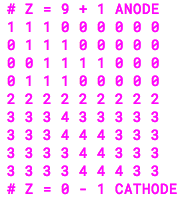
\includegraphics[width=0.3\textwidth]{Figures/device.png}
    \caption{A single slice of the test device used to write and configure the device-scale KMC code}
	\label{fig:device}
\end{figure}

\begin{center}
\begin{tabular}{| c | c | c | c |}
\hline
\rule{0pt}{2.5ex} 
\multirow{2}{*}{\textbf{ID}}&\multirow{2}{*}{\textbf{Simulation Name}}&\multirow{2}{*}{\textbf{XML Name}}&\textbf{$l_{x,y,z}$}\\
                            &&&(\SI{}{\AA})\\
\hhline{|====|}
\rule{0pt}{2.5ex}\textbf{\ccg0}&\ccg orderedP3HT&\ccg p1-L15-f0.0-P0.1-T1.5-e0.5&\ccg 85.19\\
\textbf{1}&disorderedP3HT&shrunkp1-L15-f0.0-P0.1-T2.0-e0.5&85.19\\
\textbf{\ccg2}&\ccg interfaceP3HTC60&\ccg p1-L15-f0.3-P0.1-T1.5-e0.1&\ccg 96.23\\
\textbf{3}&disorderedPCBM&pcbm-0.5-P0.5-300-T3.0\_AA&65.69\\
\textbf{\ccg4}&\ccg orderedPCBM&\ccg pcbm-0.5-P1.5-200-T5.0\_AA&\ccg 57.53\\
\hhline{----}
\end{tabular}\label{table:cells}
\captionof{table}{The morphologies selected for use in each cell in the device. The ID integers correspond to `moietyType', and `$l_{x,y,z}$' is the cubic box length for each molecular system.}
\end{center}


\begin{itemize}
    \item{The device is a cube consisting of 9x9x9 Cartesian lattice of `cells' or `moieties', where each cell in the lattice corresponds to one $\sim 10$ nm molecular morphology.}
    \item{The layout of a single x-z slice of the device is depicted in figure \ref{fig:device}. Each cell is assigned an integer [0-4], which represents the molecular morphology type within as described in table \ref{table:cells}. The structure is therefore a simple bilayer, with regions of crystalline donor and acceptor material in amongst the amorphous melt.}
    \item{9 identical copies of the slice are combined in the y-direction to make the 3D structure.}
    \item{Note that the molecular morphology describing each of these cells is actually a different size. On average, each cell represents a structure that is cubic with side 7.8 nm, and so this value was used when calculating displacements within the device.}
    \item{Additionally, no orientational manipulation has been applied to these systems. That is, that all of the P3HT crystal cells in the system are identical and oriented the same way. Similarly, the interface cells (which form vertical lamellae of P3HT in the middle and C60 molecules aggregating around the outside) have not been rotated or manipulated in any way.}
    \item{The device is periodic in the x and y directions, but is capped at $Z = -1$ and $Z = 9$ by planes that describe the cathode and anode respectively. Carriers crossing into these planes are counted towards the generated photocurrent, and excitons are forbidden from hopping into them. Eventually, these planes will also consider dark-current injection which is vital for device operation.} 
\end{itemize}

\clearpage

\section{Getting Excitons Working}

Before including carrier hopping (which will require a calculation and treatment of coulombic and field effects etc.), it is important to get the exciton dynamics correct.

\begin{itemize}
    \item{Excitons are injected into the device according to the photoinjection rate:
    \begin{equation}
        k_{\text{photo}} = \Phi \frac{\lambda}{hc} A \left( 1 - \exp^{- \alpha(z)} \right),
    \end{equation}
    where $\Phi$ is the incident flux (0.01 mW/cm$^{2}$), $\lambda$ is the wavelength (500 nm), $A$ is the photosensitive area (9 $\times$ 7.8 nm $\times$ 9 $\times$ 7.8 nm), and $\alpha$ is the thickness-dependent absorption coefficient (1.3$\times 10^4$ $\times$ 9 $\times$ 7.8 $\times 10^{-9}$)}
    \item{This rate is converted to a wait time for the next photoinjection using the normal KMC algorithm, and then an exciton is placed in a random cell, on a random chromophore after the wait time.}
    \item{Only after the exciton has been injected is the next photoinjection wait time calculated.}
    \item{The exciton is then permitted to hop based on a modified F\"orster hopping rate:
    \begin{equation}
        k_{\text{FRET}} = \frac{B}{\tau_{\text{ex}}} \left( \frac{r_{F}}{r_{ij}} \right)^{6}, 
    \end{equation}
where $\tau_{ex}$ is the exciton lifetime parameter (0.5 ns), $r_{F}$ is the F\"orster radius (4.3 nm), $r_{ij}$ is the distance from the initial chromophore to the hop destination, and $B$ is a coefficient that takes into account the Boltzmann energy penalty for hopping upstream in energy ($\exp^{- \Delta E_{ij} / k_{B} T}$ for $\Delta E_{ij} > 0$, and 1 for $\Delta E_{ij} \leq 0$), as well as a variable prefactor that will be discussed later.}
    \item{If an exciton hops to a chromophore that is within 1 nm of an opposing chromophore type (i.e. both a donor and an acceptor chromophore in range), it will instantaneously dissociate (removed from the system) to create an electron on the acceptor chromophore and a hole on the donor.}
    \item{Excitons also are given a lifetime, $t_{\text{ex}}$ based on $\tau_{\text{ex}}$ ($t_{\text{ex}} = - \ln (x \tau_{\text{ex}})$, where $x$ is a random number in the interval $[0,1)$). If the exciton would hop for any time longer than $t_{\text{ex}}$, it is instead removed from the system and counted as recombining, without generating charge carriers.}
\end{itemize}

\clearpage

\textcolor{red}{Note that all subsequent data has been run using the same random number seed to ensure comparable statistics.}

\subsection{Prefactor $= 1 \times 10^{0}$}

\begin{figure}[h!]\centering
	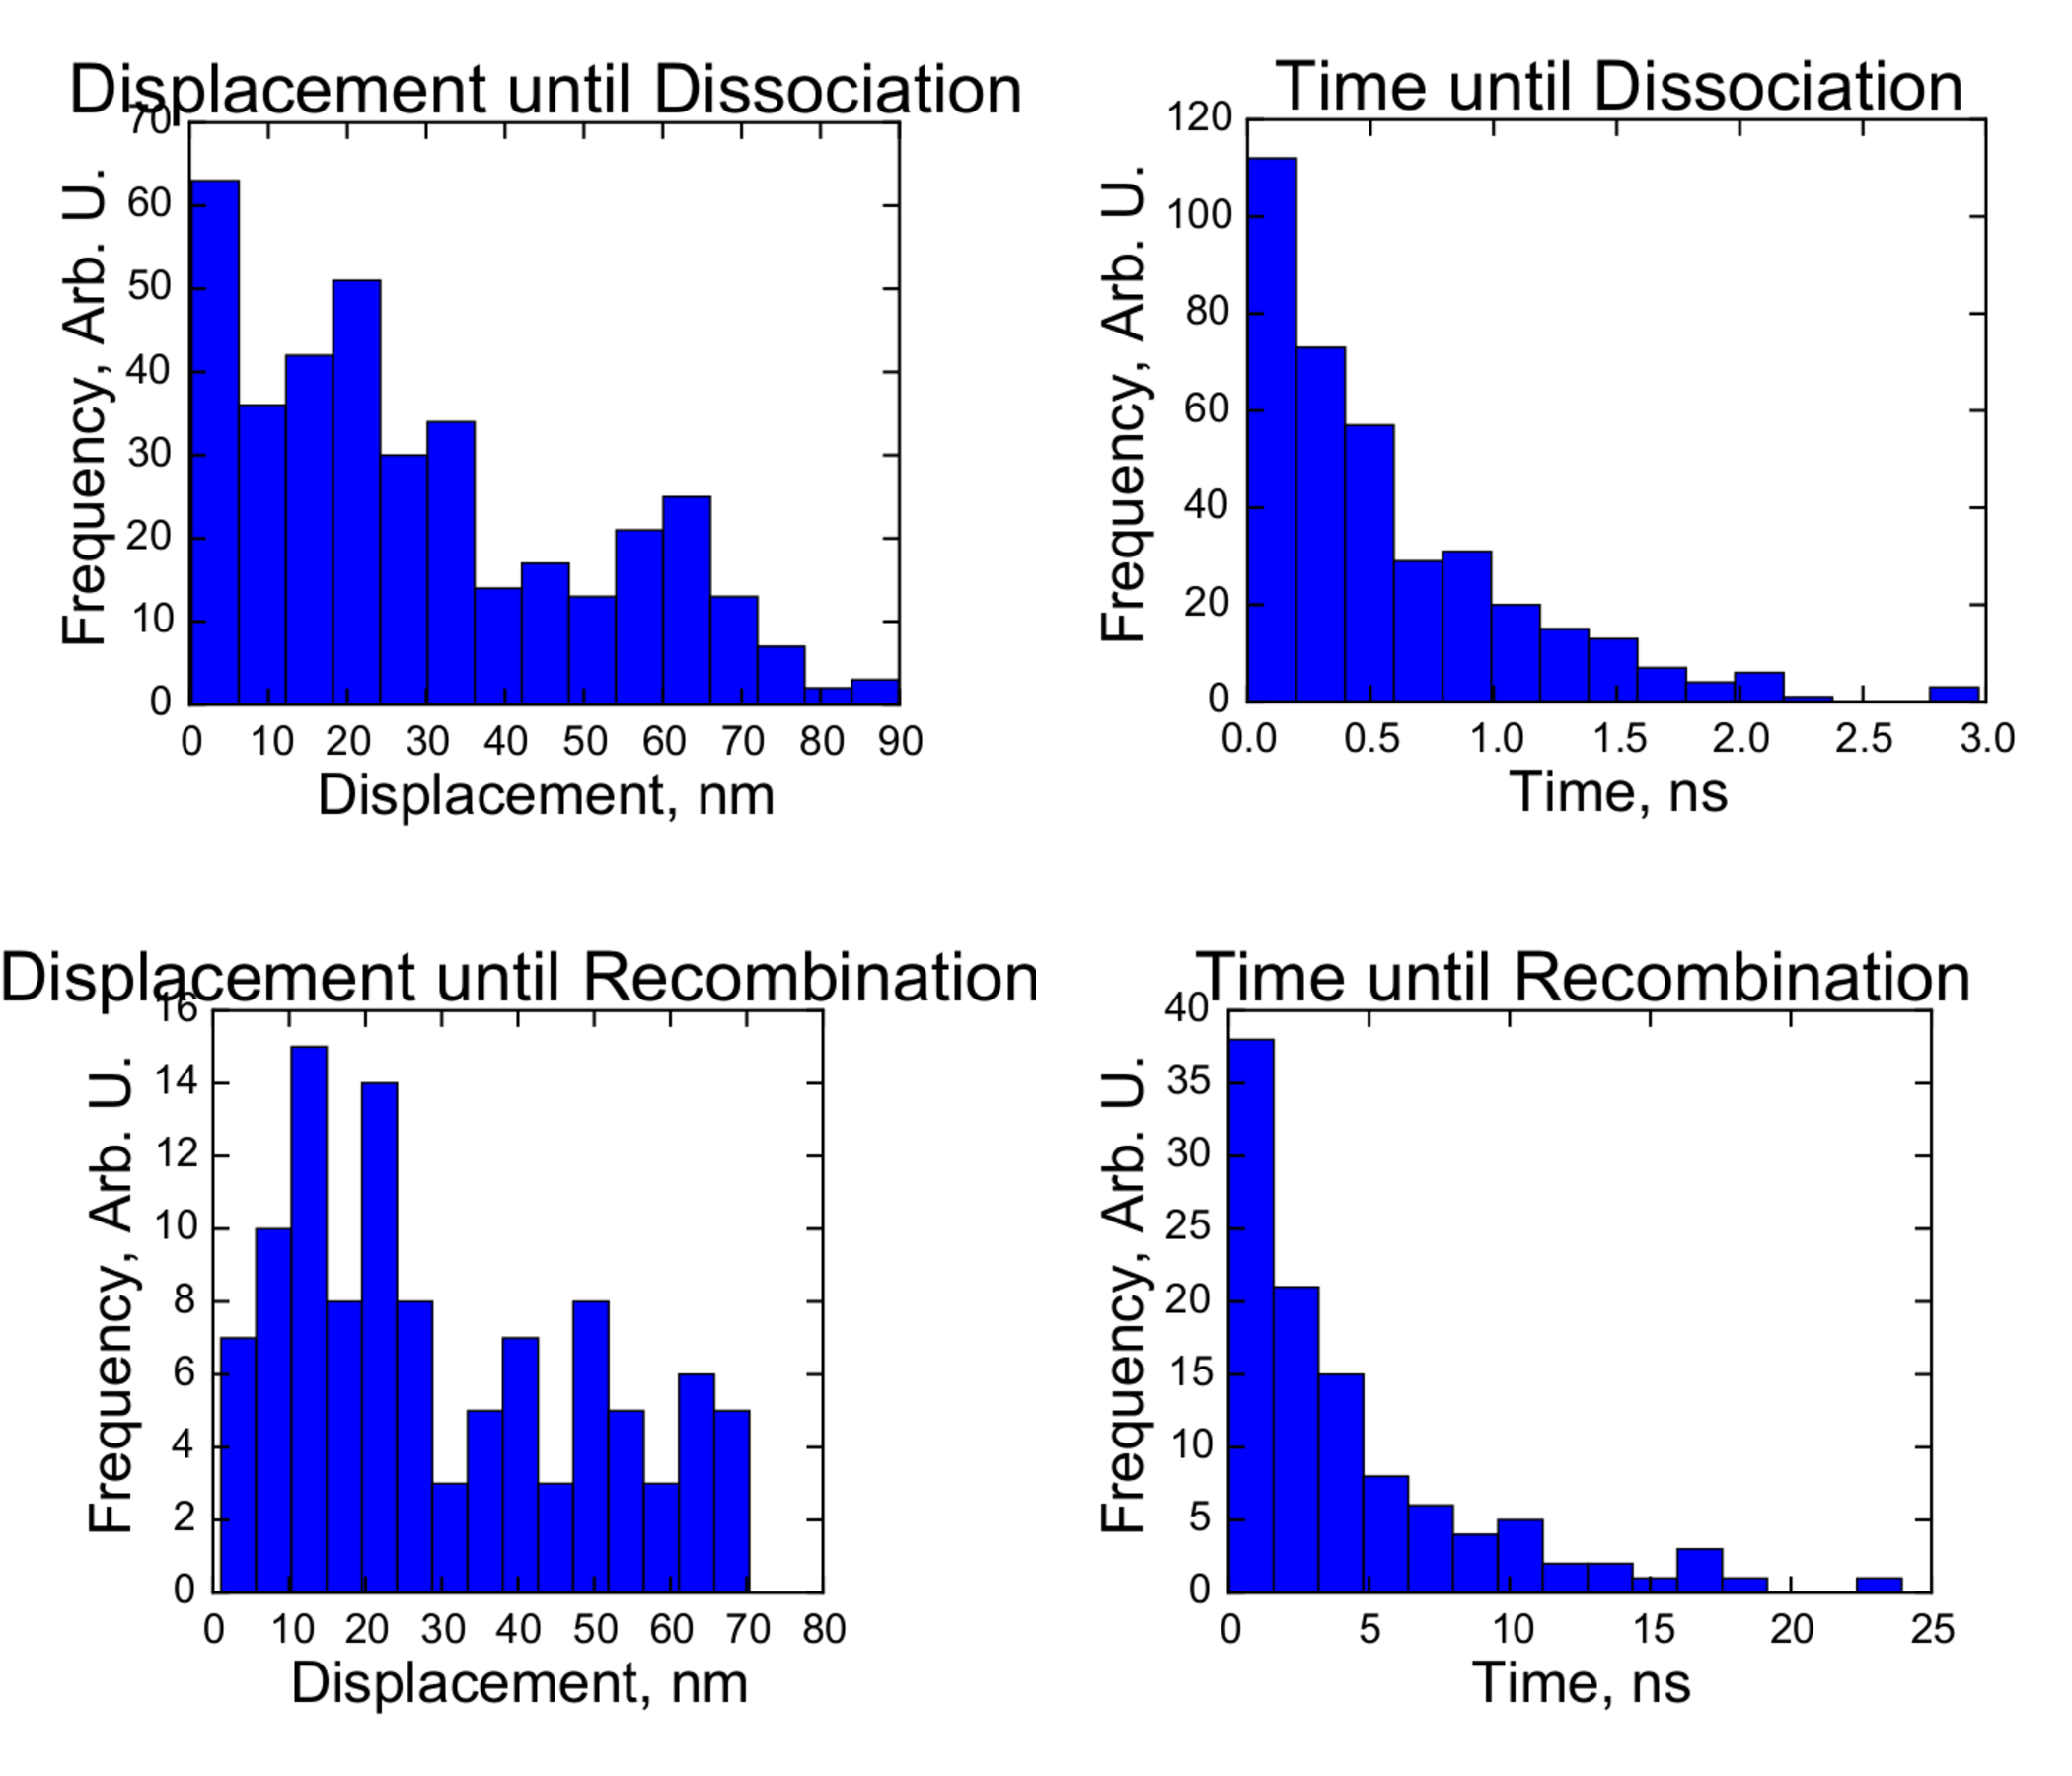
\includegraphics[width=\textwidth]{Figures/noPrefactor/noPrefactor.pdf}
    \caption{The measured exciton dynamics given a $k_{\text{FRET}}$ prefactor of 1.0}
	\label{fig:noPrefactor}
\end{figure}

\begin{itemize}
    \item{The above results incentivised the $k_{\text{FRET}}$ equation modification as it seems to be unsuitable for describing this high-resolution exciton transport.}
    \item{Excitons are consistenly moving for many tens of nm, which is too high for this kind of organic system (somewhat based on P3HT:PCBM, which has a mean-free path length of around 5 nm.}
    \item{Additionally, the lifetimes of the non-dissociating excitons are far too high. The lifetime parameter should be restricting the lifetime to around 0.5 ns, not 20+.}
    \item{The driving factor in the equation is the $(\frac{r_{F}}{r_{ij}})^{6}$. $r_{ij}$ is of the order angstroems, which forces the rate coefficient to be extremely high, allowing the exciton to move very far in a short space of time.}
    \item{As such, it might be a good idea to reduce the rate coefficient through the use of a prefactor, in order to get the expected exciton dynamics}
    \item{There is some partial justification in this according to Ref\cite{Feron2012a}, which suggests that the intrinsic point-dipole assumption in FRET might not be suitable for some materials.}
    \item{\textcolor{red}{This is a complicated issue though because Refs\cite{Athanasopoulos2009,Feron2012a} also show diffusion lengths of around 40nm given 90 meV of energetic disorder and a F\"orster length of 4.3 nm, which isn't miles off.}}
    \item{With a prefactor of 1.0, the exciton dissociation efficiency was 79\% for our bilayer morphology.}
\end{itemize}

\clearpage

\subsection{Prefactor $= 1 \times 10^{-2}$}

\begin{figure}[h!]\centering
	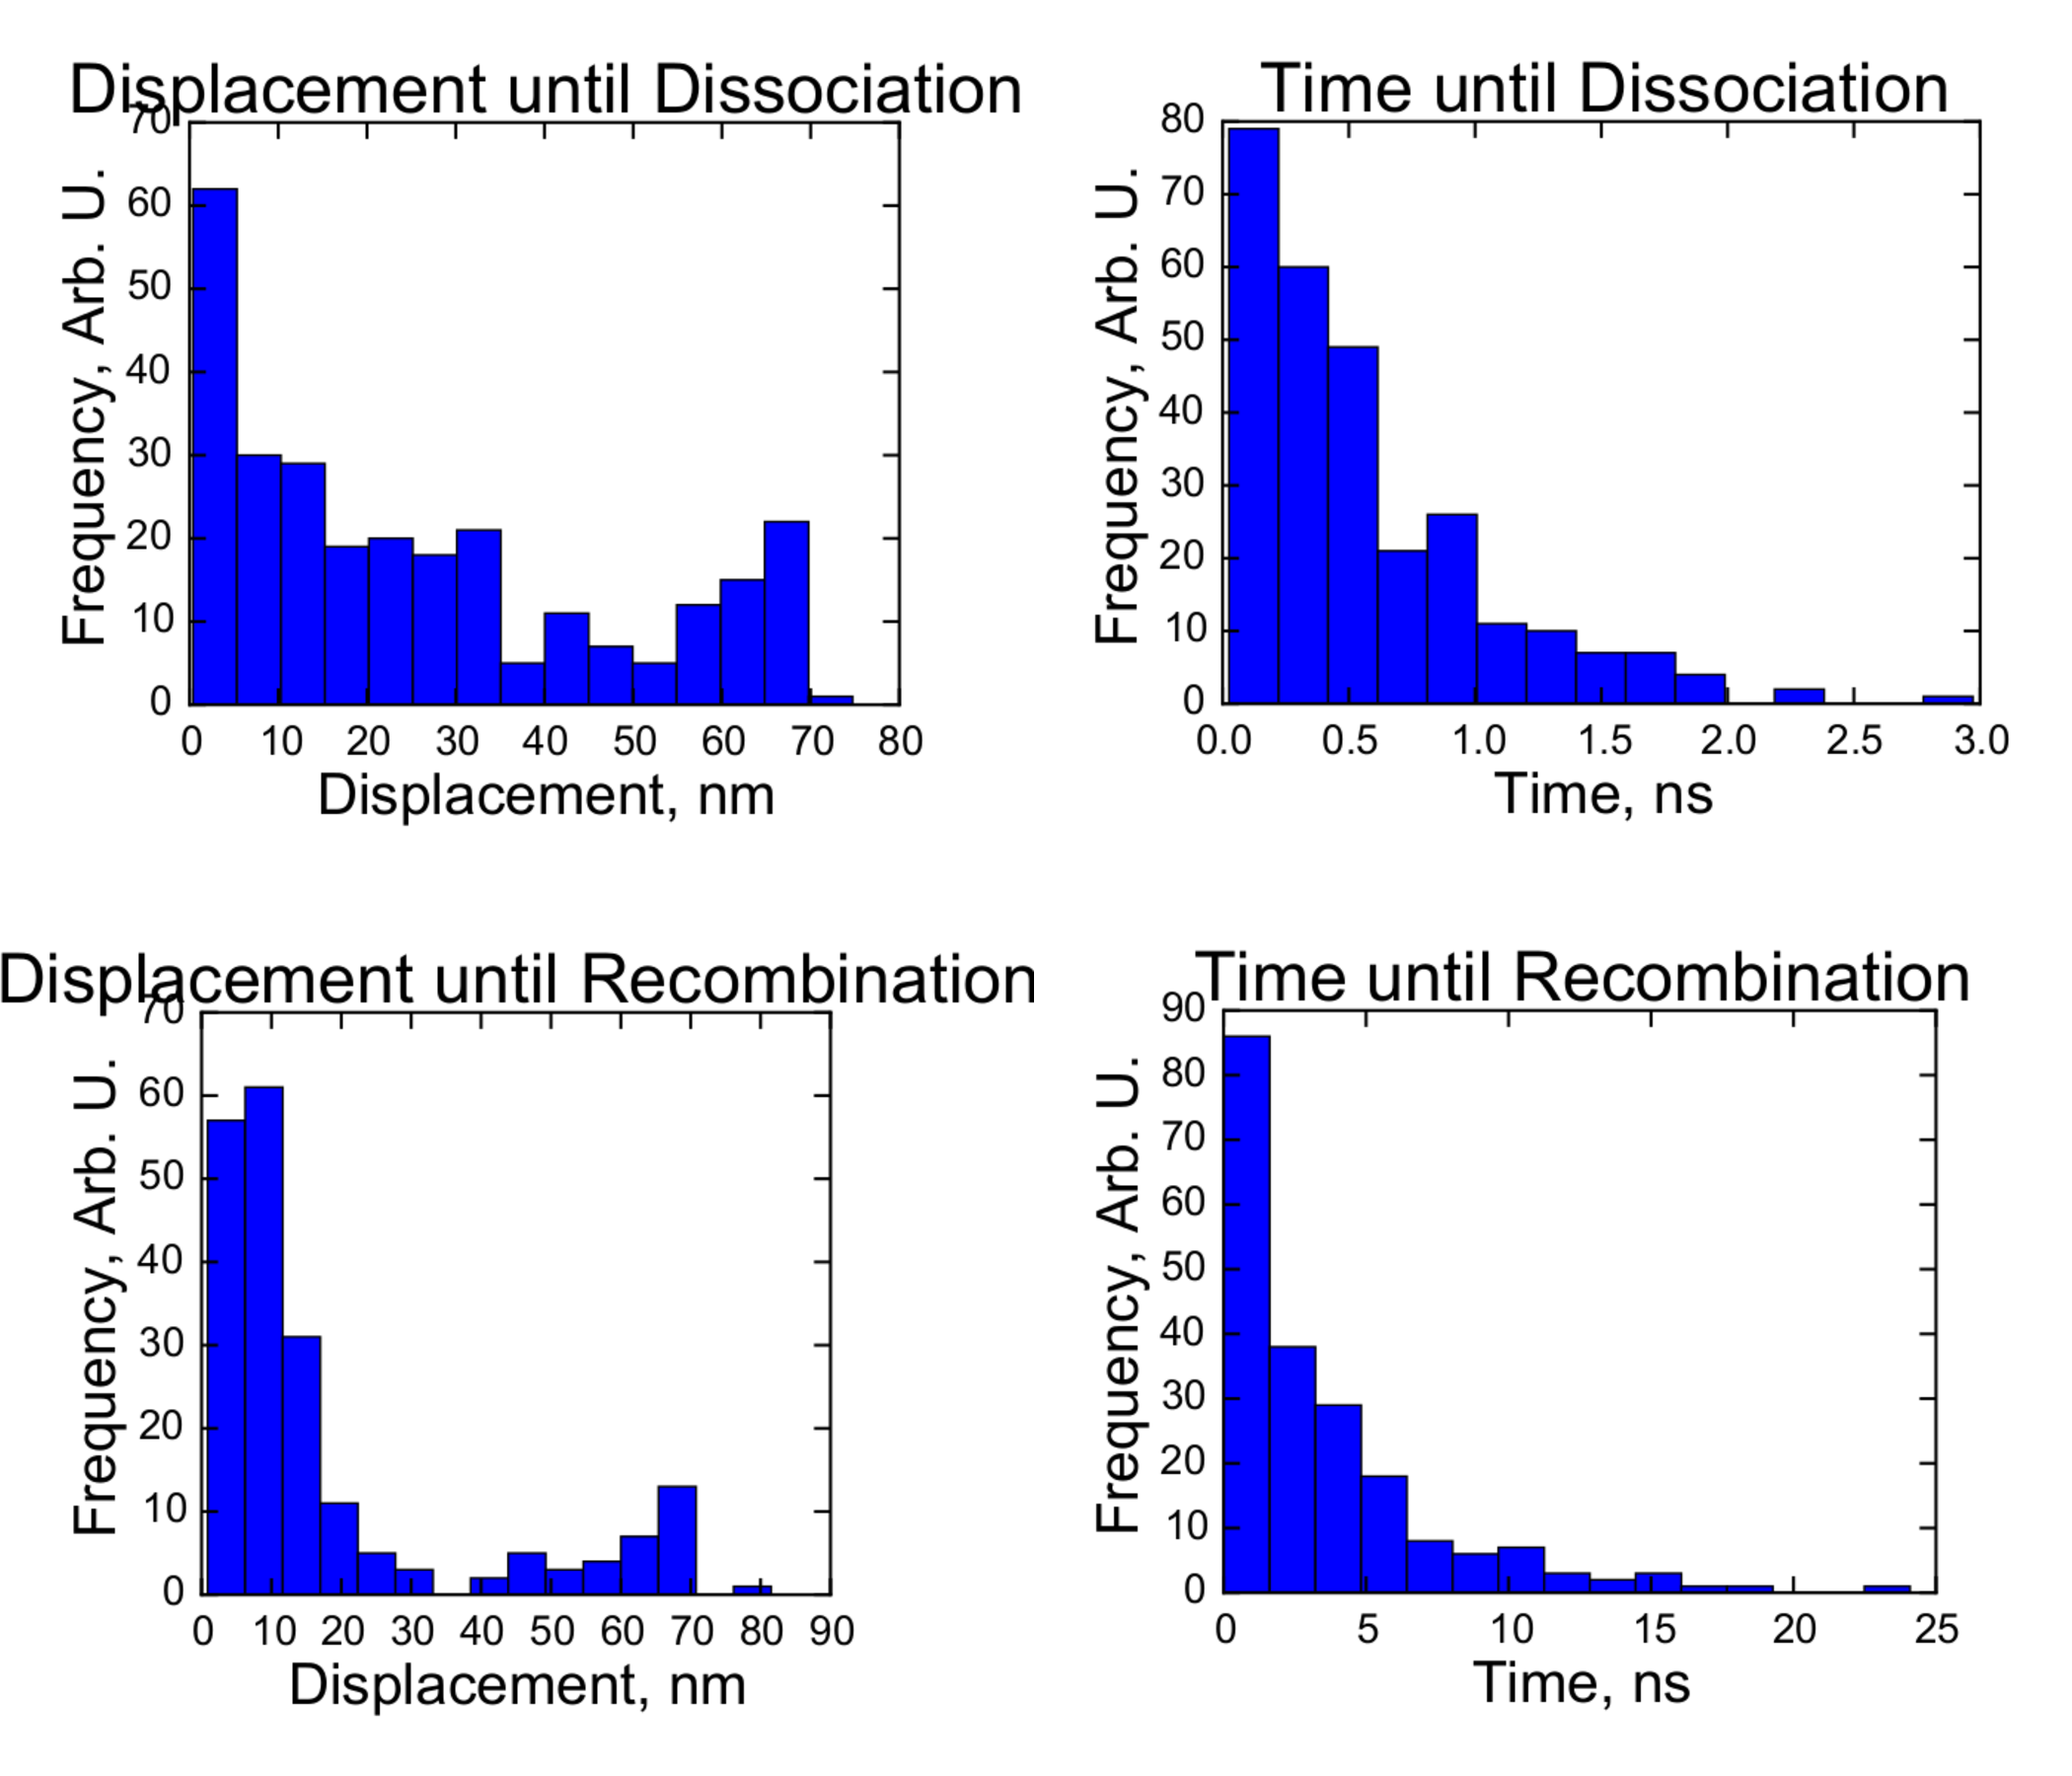
\includegraphics[width=0.9\textwidth]{Figures/prefactor01/prefactor01.pdf}
    \caption{The measured exciton dynamics given a $k_{\text{FRET}}$ prefactor of 0.01}
	\label{fig:noPrefactor}
\end{figure}

\begin{itemize}
    \item{Reducing the FRET hopping rates by 2 orders of magnitude has improved the exciton dynamics slightly, as excitons travel less far before recombining. Around twice as many excitons are recombining within 0.5 ns, and the majority have a pre-recombination free path of less then 40 nm.}
    \item{With a prefactor of 0.01, the exciton dissociation efficiency was XX\% for our bilayer morphology.}
\end{itemize}

\clearpage

\subsection{Prefactor $= 1 \times 10^{-4}$}

\begin{figure}[h!]\centering
	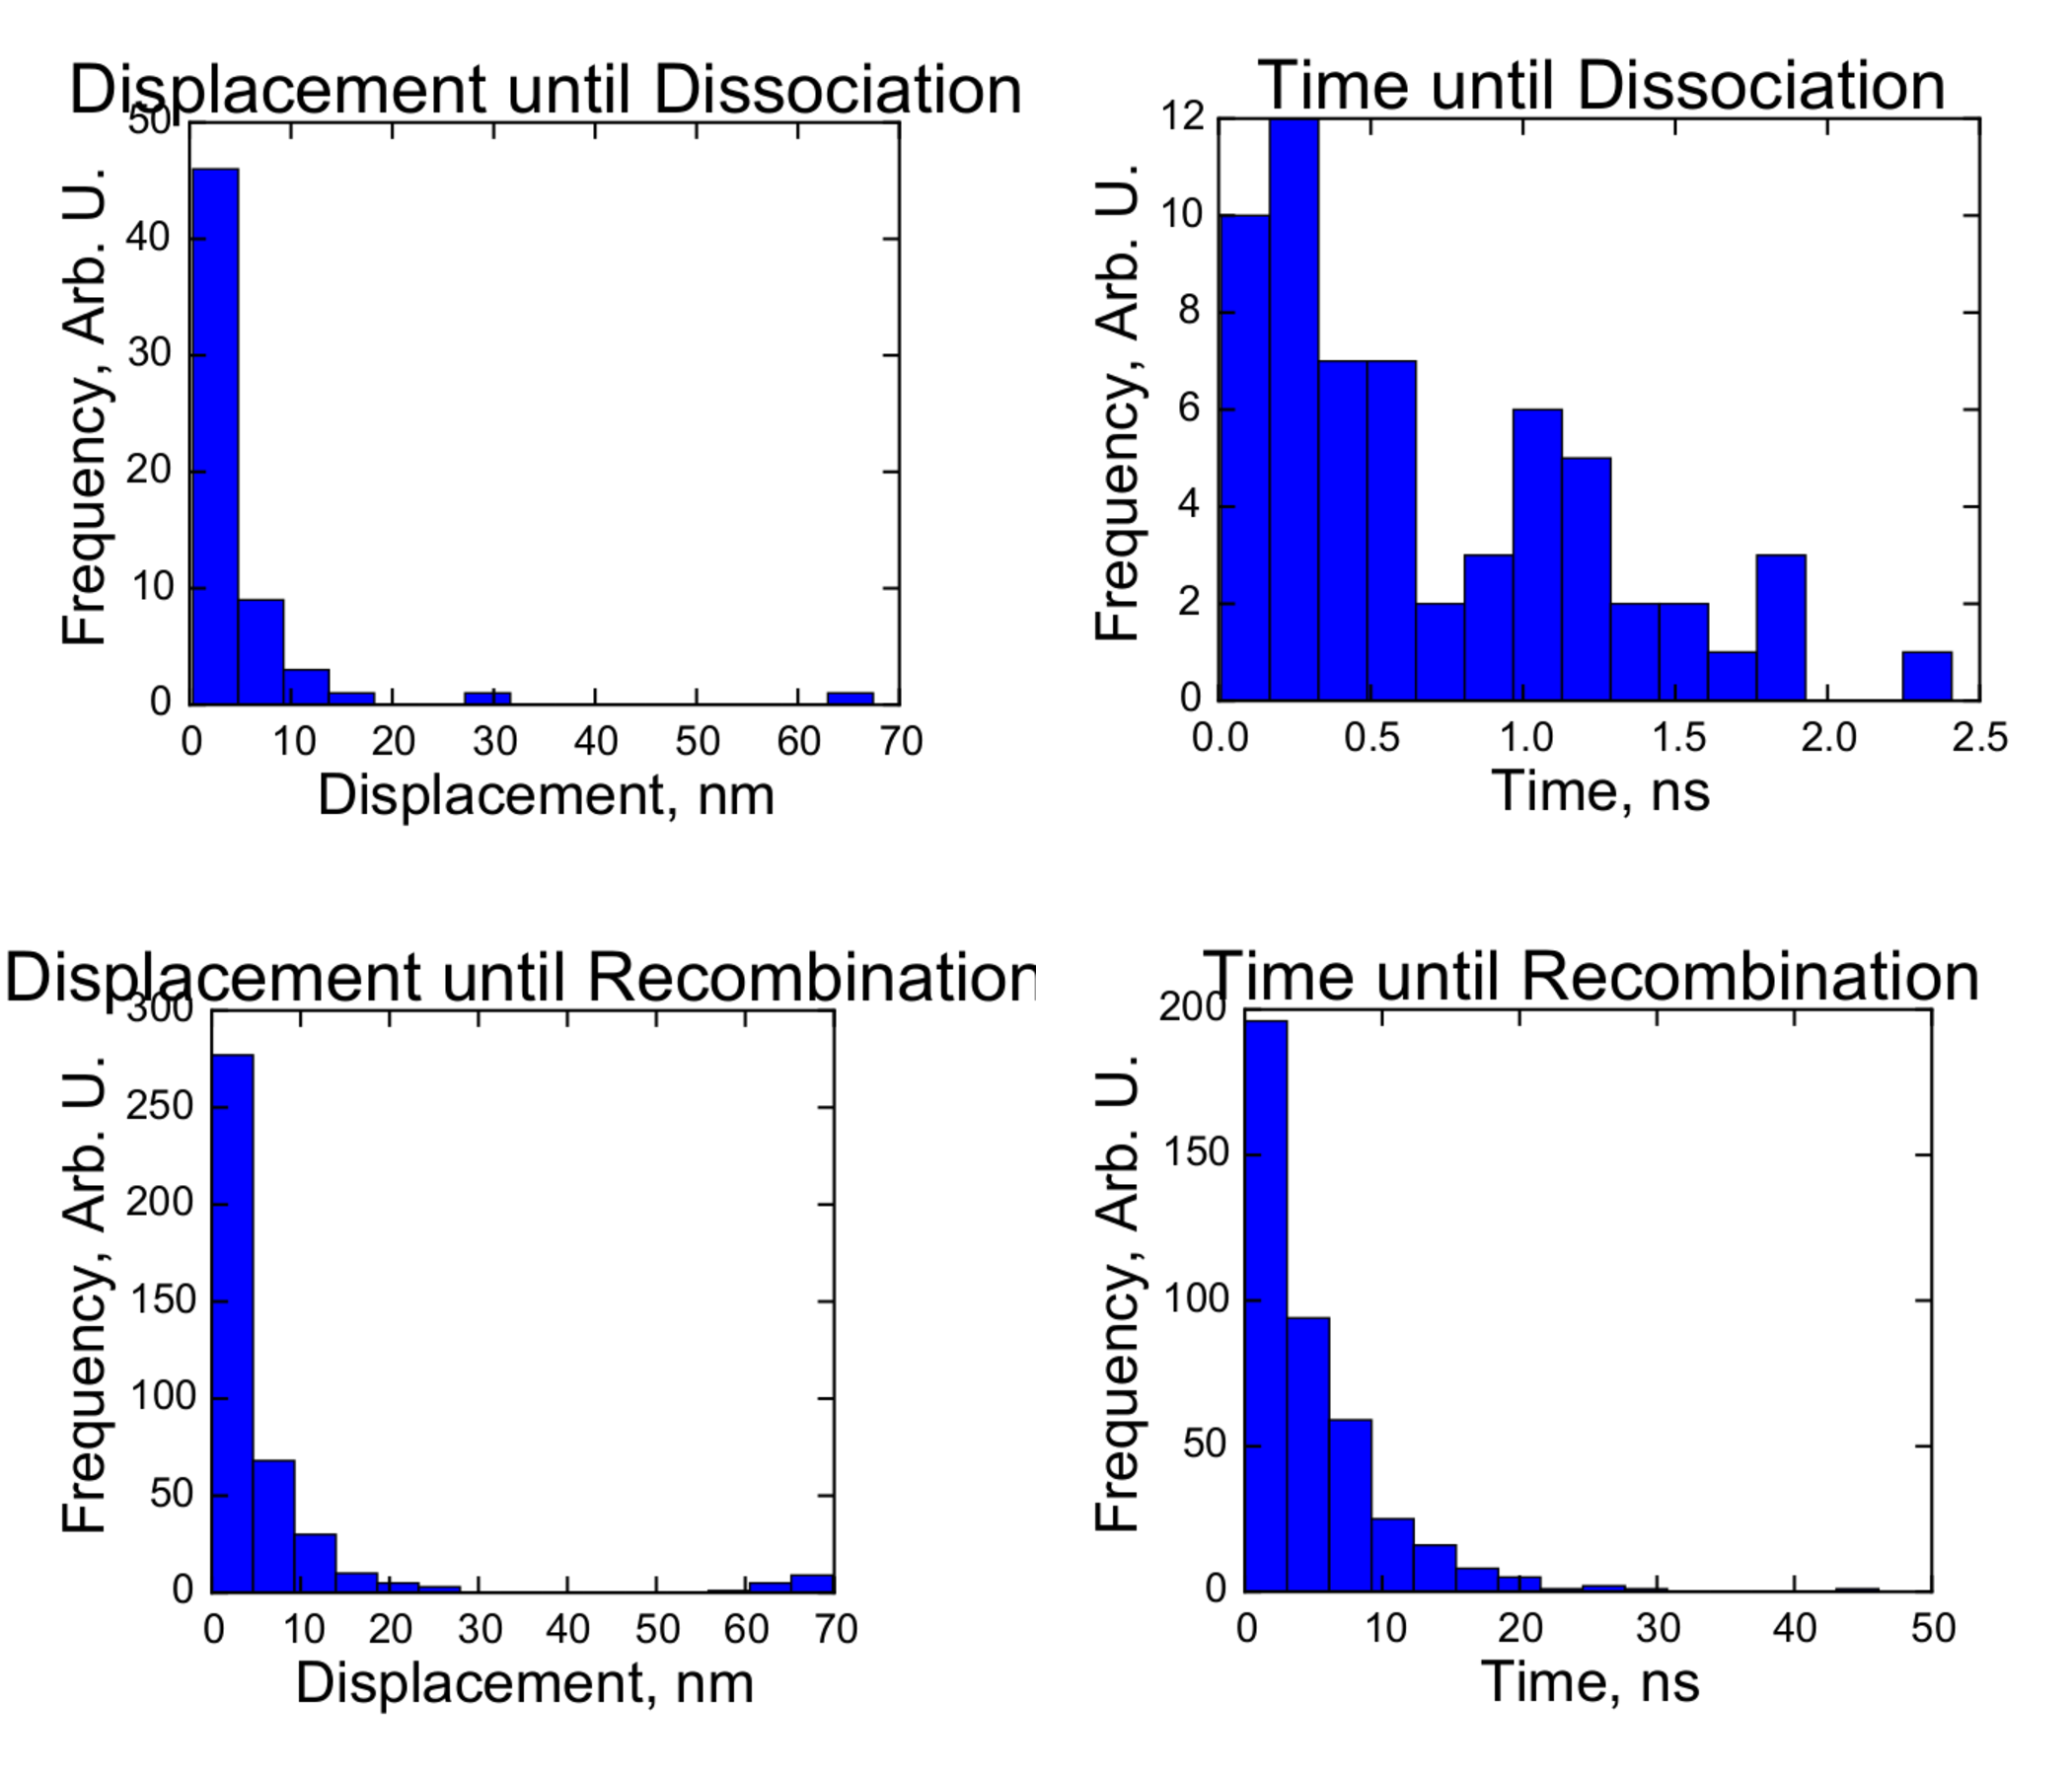
\includegraphics[width=0.9\textwidth]{Figures/prefactor0001/prefactor0001.pdf}
    \caption{The measured exciton dynamics given a $k_{\text{FRET}}$ prefactor of 0.0001}
	\label{fig:noPrefactor}
\end{figure}

\begin{itemize}
    \item{Reducing the FRET hopping rates to $1 \times 10^{-4}$ has affected the exciton dynamics more strongly, with nearly all excitons dissociating or recombining within 30 nm (except for a small few that are spawned in crystals and so can travel significantly further) and a few nanoseconds.}
    \item{With a prefactor of $1 \times 10^{-4}$, the exciton dissociation efficiency was 12.6\% for our bilayer morphology.}
\end{itemize}

\clearpage

\subsection{Summary of Prefactor Investigation}

\begin{center}
\begin{tabular}{| c | c | c | c | c | c |}
\hline
\rule{0pt}{2.5ex} 
\multirow{2}{*}{\textbf{Prefactor}}&\multicolumn{2}{| c |}{\textbf{Recombination}}&\multicolumn{2}{| c |}{\textbf{Dissociation}}&\textbf{XDE}\\
\hhline{|~-----|}
                                   &Time (ns)&Disp (nm)&Time (ns)&Disp (nm)&\%\\
\hhline{|======|}
\rule{0pt}{2.5ex}\ccg $1 \times 10^{0}$&\ccg 0.45 $\pm$ 0.04&\ccg 30 $\pm$ 2&\ccg 0.57 $\pm$ 0.03&\ccg 29 $\pm$ 1&\ccg 77.8\\
$1 \times 10^{-2}$&0.35 $\pm$ 0.03&18 $\pm$ 1&0.55 $\pm$ 0.03&26 $\pm$ 1&58.2\\
\ccg $1 \times 10^{-4}$&\ccg 0.48 $\pm$ 0.03&\ccg 6.3 $\pm$ 0.6&\ccg 0.69 $\pm$ 0.07&\ccg 5 $\pm$ 1&\ccg 12.6\\
\hhline{------}
\end{tabular}\label{table:cells}
\captionof{table}{The morphologies selected for use in each cell in the device. The ID integers correspond to `moietyType', and `$l_{x,y,z}$' is the cubic box length for each molecular system.}
\end{center}


\begin{itemize}
    \item{Modifying the prefactor does not significantly affect the average recombination or dissociation time, however, it does strongly affect the distance that the exciton can travel.}
    \item{Additionally, it significantly reduces simulation runtime, which will be important during the full carrier-included device simulations as exciton transport is not expected to be the most computationally intensive part of the simulation.}
    \item{In order to obtain the `correct' [CITATION NEEDED] path lengths for excitons in the sorts of systems that we are investigating, we should modify the F\"orster transport rate by a prefactor of $1 \times 10^{-4}$ to ensure consistent exciton dynamics.}
\end{itemize}

\clearpage

\section{Carrier Hopping $\Delta E$}

The $\Delta E$ in the Marcus hopping equation is quite different for device-scale simulations.

The following components are required:

\begin{itemize}
\item{The chromophore energy difference that was used previously ($\Delta E_{ij}$ - note that this is 0 for small molcules, so it might be important to add some energetic disorder to this if we deem it necessary)}
\item{The drift component.
        Now that we're simulating a full device, there is a potential within the system that biases hops along the $z$-axis due to the potential applied across the electrical contacts.
        As the field increases, electrons are forced through the anode, which reduces the number of extractions and therefore the ouput current of the device.
    Holes are forced in the opposite direction.}
\item{Finally, since we are now simulating more than one charge carrier, the Coulombic effects of nearby carriers must be taken into account.
    The Durham code also includes image charges, and I've put in the infrastructure for this, but I don't really understand their prescence properly, so I'm trying without them for now to see what we get.
    I'll dig into Ben and Chris' old papers to learn more about these images.}
\end{itemize}

These components will probably need a lot more testing, but preliminary data shows the following magnitudes for these components:

\begin{itemize}
    \item{The $\Delta E_{ij}$ component has a magnitude of several hundred meV, unless we're dealing with hopping between small molecules (i.e. identical chromophores) in which case $\Delta E_{ij} = 0$.}
    \item{The drift component is pretty small. In the case of an applied voltage of 0.2 (corresponding to a field of around $1 \times 10^{7}$ Vm$^{-1}$), the component contribues $\sim 1$ meV to the $\Delta E$.
        This could be on the small side, or it could be exactly right - I just don't know.
        One thing I can do is take a look at the Durham data (on my laptop) to see if we ever output those magnitudes anywhere that might be able to give me some idea of if this is correct or not.}
    \item{The Coulombic effects have a magnitude of several hundred meV (for immediately dissociated carriers), and it feels sensible that the Coulomb potential is of similar order to the energetic disorder arising from chromophore fluctuations.}
\end{itemize}
\clearpage


\section{KMC Timescales}


\begin{itemize}
    \item{A Fermi-estimate of the timescales involved in the KMC indicated that the carrier hops in P3HT (tons of single-monomer chromophores that are super close together) suggested that we were spanning $\sim 16$ orders of magnitude in time between our fastest and slowest events, from $1 \times 10^{-18}$ s for the fastest carrier hops and $1 \times 10^{-2}$ s for the photoinjections.}
    \item{Perhaps we can use the FRET hopping prefactor here to slow down the carrier hops as well, given that we justify the prefactor due to the tiny hops that occur between the densely packed chromophores. \textcolor{red}{Using this prefactor slows down the mobilities that we obtained using the molecular KMC}. The advantage is that this saves 4 orders of magnitude, bringing the difference down to 12.}
    \item{The incident flux was set to 0.01 mW/cm$^{2}$ rather than the 100 mW/cm$^{2}$ that correctly corresponds to AM1.5. This reduces the number of orders of magnitude by another 4 to 8.}
\end{itemize}

\begin{figure}[h!]\centering
	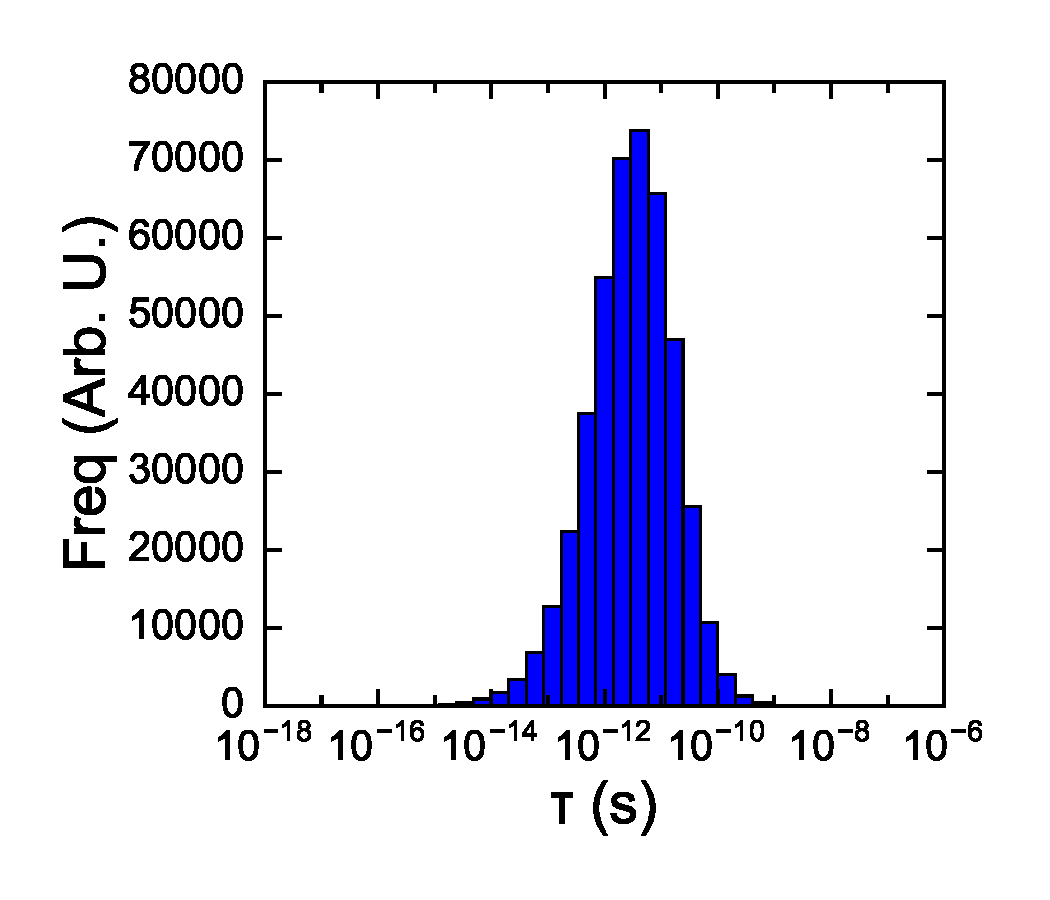
\includegraphics[width=0.5\textwidth]{Figures/EventTimeDist.pdf}
    \caption{The distribution of the event timescales observed in a device simulation consisting of around 500,000 KMC iterations (corresponding to 23 photoinjections)}
	\label{fig:eventTimeDist}
\end{figure}

\begin{itemize}
    \item{Figure \ref{fig:eventTimeDist} shows the resultant distribution of timescales in the device simulations, after about 500,000 iterations ($\sim 15$ minutes of runtime).}
    \item{The following data can be obtained from the distribution:
        \begin{itemize}
            \item{Slowest Event = $5.00 \times 10^{-6}$ s}
            \item{Fastest Event = $1.21 \times 10^{-17}$ s}
            \item{Mean = $5.40 \times 10^{-11}$ s}
            \item{STD = $1.04 \times 10^{-8}$ s}
        \end{itemize}
    }
\item{The results show a computationally tangible distribution of event times. While the range is still 11 orders of magnitude, the vast majority of events occur between 10$^{-13}$ and 10$^{-10}$ s.}
\end{itemize}



\bibliography{refs}
\bibliographystyle{unsrt}


\end{document}
